Постановка авторегрессионнного моделирования, включающая предсказание следующего слова по предшествующему контексту,
может быть использована для решения ключевых для обработки языка задач перевода, пересказа и выделения ключевых слов. 
При этом требуется задание необходимой текстовой структуры. Данная техника позволила исследователям \cite{radford2021learning} обучить
общую модель работы с текстом GPT (генеративный обучающий трансформер). Отличительной особенностью исследования была его
масштабность. Модель обучена на объеме более триллиона слова, полученного с помощью выделения естественного языка из источников в internet.
Таким образом, в краткие сроки были приобретены навыки языка на более чем ста языках мира и базовые знания об естественных и социальных науках.
Для прохождения испытаний по метрической оценке навыков модели были использованы корпуса высокого качества. 

\begin{figure}[h]
    \centering
    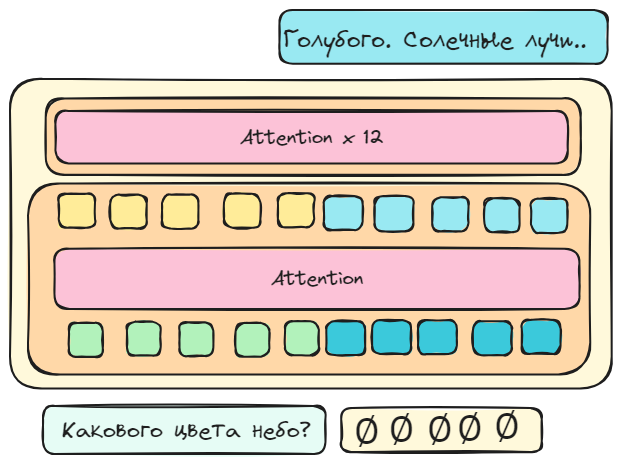
\includegraphics[width=0.5\textwidth]{assets/ml/nlp/gpt.excalidraw.png}
    \caption{GPT обучается как авторегрессионная модель на ко}
    \label{gpt}
\end{figure}

Обучение языковых моделей для задач ассистирования разделяется на два этапа предобучение (\textit{англ.} pretrain) и инструкционное дообучение.
В ходе первого этапа модель обучается синтаксической структуре языка. Нао втором этапе модель обучается под руководством эксперта на 
специализированных корпусах инструкций. Таковыми, например, могут являться выдача структурированных определений, изложение информации в требуемой
стилистической форме, поиск ключевых слов в большом по объему тексте.

\begin{figure}[h]
    \centering
    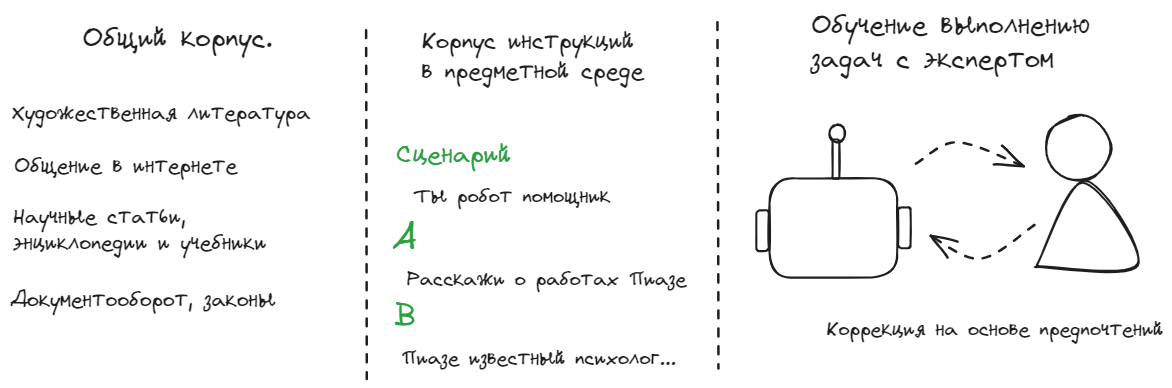
\includegraphics[width=0.5\textwidth]{assets/work/arch/learning.excalidraw.png}
    \caption{Обучение разбито на три ключевых этапа: подготовка, адаптация на корпусе.}
    \label{train}
\end{figure}

Предобучение требует значительных вычислительных ресурсов, не всегда доступных в образовательных и научных
приложениях. В связи с этим компании, обладающие достаточным ресурсом, делают свои модели общедоступными \cite{jiang2023mistral} \cite{jiang2024mixtral} \cite{touvron2023llama}

Для оценки способностей языковых моделей создаются специальные системы тестирования, количественно оценивающие способности моделей к:
\begin{itemize}
    \item способности к пересказу и перевода;
    \item пониманию животного и растительного мира;
    \item социальных правил и законов;
    \item решение аналитических задач.
\end{itemize}

\begin{figure}[h]
    \centering
    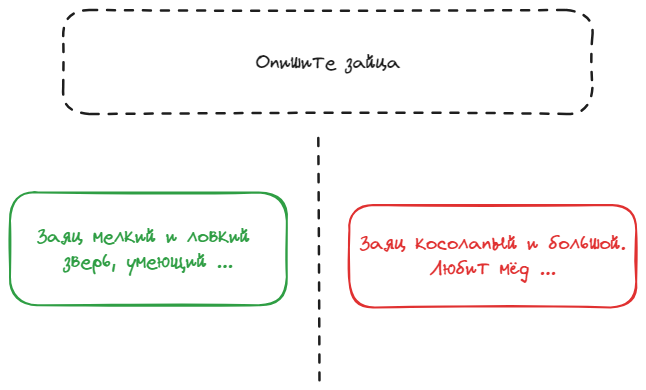
\includegraphics[width=0.5\textwidth]{assets/work/arch/instruction.excalidraw.png}
    \caption{Адаптация к задачам выполняется путем взаимодействия с пользователем и работой с экспертом.}
    \label{instruction}
\end{figure}

Для сравнения моделей также используется техника попарного сравнения моделей. Таким образом, исходя из предпочтений пользователей, 
выносится оценка модели.

Большие языковые модели не гарантируют корректное исполнение даже базовых арифметических операций. В обзоре \cite{zhao2023survey} показано, 
что подобные проблемы возникают во многих строгих постановках, где соблюдение формы требует интеллектуального участия 
\begin{itemize}
    \item написание исполняемого языком программирования кода;
    \item переход в математических выражениях.
\end{itemize} 

Для решения проблемы исследователи предложили использование инструментов, которые используются моделью для качественного
выполнения инструкции. На данный момент сложились следующие подходы:
\begin{itemize}
    \item обращения к информационным системам (RAG - retreival augmented generation)\cite{lewis2020retrieval};
    \item работа с средой исполнения программного кода \cite{parisi2022talm};
    \item генерация сопровождающей иллюстрации \cite{rombach2022high}.
\end{itemize}










